%%%%%%%%%%%%%%%%%%%%%%%%%%%%%%%%%%%%%%%%%
% Wenneker Assignment
% LaTeX Template
% Version 2.0 (12/1/2019)
%
% This template originates from:
% http://www.LaTeXTemplates.com
%
% Authors:
% Vel (vel@LaTeXTemplates.com)
% Frits Wenneker
%
% License:
% CC BY-NC-SA 3.0 (http://creativecommons.org/licenses/by-nc-sa/3.0/)
% 
%%%%%%%%%%%%%%%%%%%%%%%%%%%%%%%%%%%%%%%%%

%----------------------------------------------------------------------------------------
%	PACKAGES AND OTHER DOCUMENT CONFIGURATIONS
%----------------------------------------------------------------------------------------

\documentclass[11pt]{scrartcl} % Font size

%%%%%%%%%%%%%%%%%%%%%%%%%%%%%%%%%%%%%%%%%
% Wenneker Assignment
% Structure Specification File
% Version 2.0 (12/1/2019)
%
% This template originates from:
% http://www.LaTeXTemplates.com
%
% Authors:
% Vel (vel@LaTeXTemplates.com)
% Frits Wenneker
%
% License:
% CC BY-NC-SA 3.0 (http://creativecommons.org/licenses/by-nc-sa/3.0/)
% 
%%%%%%%%%%%%%%%%%%%%%%%%%%%%%%%%%%%%%%%%%

%----------------------------------------------------------------------------------------
%	PACKAGES AND OTHER DOCUMENT CONFIGURATIONS
%----------------------------------------------------------------------------------------

\usepackage{amsmath, amsfonts, amsthm} % Math packages

\usepackage{listings} % Code listings, with syntax highlighting

\usepackage[english]{babel} % English language hyphenation

\usepackage{graphicx} % Required for inserting images
\usepackage{caption}
\graphicspath{{Figures/}{./}} % Specifies where to look for included images (trailing slash required)

\usepackage{booktabs} % Required for better horizontal rules in tables

\numberwithin{equation}{section} % Number equations within sections (i.e. 1.1, 1.2, 2.1, 2.2 instead of 1, 2, 3, 4)
\numberwithin{figure}{section} % Number figures within sections (i.e. 1.1, 1.2, 2.1, 2.2 instead of 1, 2, 3, 4)
\numberwithin{table}{section} % Number tables within sections (i.e. 1.1, 1.2, 2.1, 2.2 instead of 1, 2, 3, 4)

\setlength\parindent{0pt} % Removes all indentation from paragraphs

\usepackage{enumitem} % Required for list customisation
\setlist{noitemsep} % No spacing between list items

%----------------------------------------------------------------------------------------
%	DOCUMENT MARGINS
%----------------------------------------------------------------------------------------

\usepackage{geometry} % Required for adjusting page dimensions and margins

\geometry{
	paper=a4paper, % Paper size, change to letterpaper for US letter size
	top=2.5cm, % Top margin
	bottom=3cm, % Bottom margin
	left=3cm, % Left margin
	right=3cm, % Right margin
	headheight=0.75cm, % Header height
	footskip=1.5cm, % Space from the bottom margin to the baseline of the footer
	headsep=0.75cm, % Space from the top margin to the baseline of the header
	%showframe, % Uncomment to show how the type block is set on the page
}

%----------------------------------------------------------------------------------------
%	FONTS
%----------------------------------------------------------------------------------------

\usepackage[utf8]{inputenc} % Required for inputting international characters
\usepackage[T1]{fontenc} % Use 8-bit encoding

\usepackage{fourier} % Use the Adobe Utopia font for the document

%\usepackage[framed,numbered,autolinebreaks,useliterate]{mcode}

%----------------------------------------------------------------------------------------
%	SECTION TITLES
%----------------------------------------------------------------------------------------

\usepackage{sectsty} % Allows customising section commands

\sectionfont{\normalfont\bfseries} % \section{} styling
\subsectionfont{\normalfont\bfseries} % \subsection{} styling
\subsubsectionfont{\normalfont\itshape} % \subsubsection{} styling
\paragraphfont{\normalfont\scshape} % \paragraph{} styling

%----------------------------------------------------------------------------------------
%	HEADERS AND FOOTERS
%----------------------------------------------------------------------------------------

\usepackage{scrlayer-scrpage} % Required for customising headers and footers

\ohead*{} % Right header
\ihead*{} % Left header
\chead*{} % Centre header

\ofoot*{} % Right footer
\ifoot*{} % Left footer
\cfoot*{\pagemark} % Centre footer

% MY PACKAGES
%\usepackage[framed,numbered,autolinebreaks,useliterate]{mcode}
\usepackage{listings}
\usepackage{float}
\usepackage{amsmath}
\usepackage{tikz}
\usetikzlibrary{shapes,arrows,positioning}
\usepackage{hyperref} % Include the file specifying the document structure and custom commands

%----------------------------------------------------------------------------------------
%	TITLE SECTION
%----------------------------------------------------------------------------------------

\title{	
	\normalfont\normalsize
	\textsc{Universität Würzburg}\\ % Your university, school and/or department name(s)
	\vspace{25pt} % Whitespace
	\rule{\linewidth}{0.5pt}\\ % Thin top horizontal rule
	\vspace{20pt} % Whitespace
	{\huge Übung 7}\\ % The assignment title
	{\Large Ausgangsrückführung, LQR}\\
	\vspace{12pt} % Whitespace
	\rule{\linewidth}{2pt}\\ % Thick bottom horizontal rule
	\vspace{12pt} % Whitespace
}

\author{\LARGE Alexander Björk, Janis Kaltenthaler} % Your name

\date{\normalsize\today} % Today's date (\today) or a custom date

\begin{document}

\maketitle % Print the title

\tikzstyle{block} = [draw, fill=blue!20, rectangle, 
    minimum height=3em, minimum width=6em]
\tikzstyle{sum} = [draw, fill=blue!20, circle, node distance=1cm]
\tikzstyle{input} = [coordinate]
\tikzstyle{output} = [coordinate]
\tikzstyle{pinstyle} = [pin edge={to-,thin,black}]
\newcommand{\inte}{$\displaystyle \int$}

\section*{Aufgabe 7-1. Ausgangsrückführung (5 Punkte)}
\subsection*{a)}
Damit die Pole des geschlossenen Regelkreises bei den geforderten Werten liegen, ergibt sich durch die Berechnung in Matlab die folgende Regelmatrix:
\begin{align*}
	K_x=\begin{bmatrix}1.6205\\-1.41\end{bmatrix}
\end{align*}
Der Vorfilter $V$ wird nun wie folgt bestimmt:
\begin{align*}
	V_x=-\bigl(C(A-BK_x)^{-1}B\bigr)^{-1}=0.052632
\end{align*}
Das resultierende Zustandsraummodell mit Zustandsrückführung erhält man nun wie folgt:
\begin{align*}
	\dot{x}(t)&=(A-BK_x)x(t)+BV_xw(t)=\begin{bmatrix}-0.24100&-0.17993\\-2.16205&-2.85900\end{bmatrix}x(t)+\begin{bmatrix}0.1052632\\0.0052632\end{bmatrix}w(t)\\
	y(t)&=Cx(t)=\begin{bmatrix}1&0\end{bmatrix}
\end{align*}
\subsection*{b)}
Das System mit Ausgangsrückführung ist stabil, falls alle Pole des geschlossenen Regelkreis mit Ausgangsrückführung einen negativen Realteil besitzen. Um dies zu Prüfen nutzen wir das Hurwitz-Kriterium. Die System Matrix $\bar{A}$ des geschlossenen Regelkreises berechnet sich wie folgt:
\begin{align*}
	\bar{A}=A-Bk_yC=\begin{bmatrix}3-2\cdot k_y&-3\\-0.1\cdot k_y-2&-3 \end{bmatrix}
\end{align*}
Das charakteristische Polynom des geschlossenen Regelkreises berechnet sich wie folgt:
\begin{align*}
	\text{det}(\bar{A}-\lambda I)=\underbrace{1}_{a_0}\cdot\lambda^2+\underbrace{2\cdot k_y}_{a_1}\cdot\lambda+\underbrace{5.7\cdot k_y-15}_{a_2}
\end{align*}
Daraus ergibt sich die Hurwitzmatrix:
\begin{align*}
	H=\begin{bmatrix}a_1&a_3\\a_0&a_2 \end{bmatrix}=\begin{bmatrix}2\cdot k_y&0\\1&5.7\cdot k_y-15 \end{bmatrix}
\end{align*}
Die zwei Hauptabschnittsdeterminanten $D_1$ und $D_2$ werden wie folgt berechnet:
\begin{align*}
	D_1&=a_1=2\cdot k_y\\
	D_2&=\text{det}\Biggl(\begin{bmatrix}2\cdot k_y&0\\1&5.7\cdot k_y-15 \end{bmatrix}\Biggr)=2\cdot k_y\cdot(5.7\cdot k_y-15)
\end{align*}
Das betrachtete System ist stabil falls alle Koeffizienten $a_i$ und alle Hauptabschnittsdeterminanten $D_i$ positiv sind. Daher ist das System stabil für $k_y>\frac{15}{5.7}\approx2.63$ und somit durch eine Ausgangsrückführung stabilisierbar.
\subsection*{c)}
Zuerst prüfen wir ob die Zustandsrückführung durch eine Ausgangsrückführung ersetzt werden kann:
\begin{align*}
	\text{Rang}\begin{bmatrix}C\\K\end{bmatrix}=2\neq\text{Rang }C=1
\end{align*}
Da die Ränge nicht gleich sind ist eine direkte Ersetzung nicht möglich.\\
Nun berechnen wir die Eigenvektormatrix $\bar{V}$ von $A-BK_x$:
\begin{align*}
	V=\begin{bmatrix}0.787112&0.065079\\-0.616810&0.997880\end{bmatrix}
\end{align*}
Die Wichtungsmatrix $W$ wird wie folgt definiert:
\begin{align*}
	W=\begin{bmatrix}1&0\\0&1\end{bmatrix}
\end{align*}
Nun ermitteln wir die Ausgangsrückführung $K_y$ nach Gleichung:
\begin{align*}
	k_y=KVW(CVW)^T\bigl((CVW)(CVW)^T\bigr)^{-1}=2.5712
\end{align*}
Um zu Prüfen ob die Güteforderungen erfüllt werden, d.h. ob das resultierende System stabil ist, berechnen wir die Eigenwerte der Systemmatrix $A-Bk_yC$:
\begin{align*}
	\lambda_1=0.066126,\hspace{3pt}\lambda_2=-5.208437
\end{align*}
Wegen $\lambda_1>0$ ist das System nicht stabil. Entsprechend passen wir die Wichtungsfunktion an, damit $\lambda_1$ genauer an den geforderten Eigenwert von $-0.1$ angenähert wird:
\begin{align*}
	W=\begin{bmatrix}2&0\\0&1\end{bmatrix}
\end{align*}
Nun erhalten wir eine Ausgangsrückführung von:
\begin{align*}
	k_y=2.6867
\end{align*}
mit den Eigenwerten:
\begin{align*}
	\lambda_1=-0.059103,\hspace{3pt}\lambda_2=-5.314262
\end{align*}
Das System ist nun dementsprechend stabil.\\
Der Vorfilter $V_y$ zur Sicherung der Sollwertfolge bei der Ausgangsrückführung berechnet sich wie folgt:
\begin{align*}
	V_y=-\bigl(C(A-Bk_yC)^{-1}B\bigr)^{-1}=0.055103
\end{align*}
Das resultierende Zustandsraummodell mit Ausgangsrückführung erhält man nun wie folgt:
\begin{align*}
	\dot{x}(t)&=(A-BK_yC)x(t)+BV_yw(t)=\begin{bmatrix}-2.3734&-3.0000\\-2.2687&-3.0000\end{bmatrix}x(t)+\begin{bmatrix}0.1102067\\0.0055103\end{bmatrix}w(t)\\
	y(t)&=Cx(t)=\begin{bmatrix}1&0\end{bmatrix}
\end{align*}
\section*{Aufgabe 7-2. LQ-Regler (3 Punkte)}
\subsection*{a)}
Die LQ-Regelung kann angewendet werden falls das System vollständig steuerbar ist.\\
Um auf Steuerbarkeit zu Prüfen berechnen wir zunächst die Steuerbarkeitsmatrix $S_S$:
\begin{align*}
	S_S=\begin{bmatrix}b&Ab\end{bmatrix}=\begin{bmatrix}0&1\\1&4\end{bmatrix}
\end{align*}
Nach dem Steuerbarkeitskriterium von Kalman ist das System vollständig steuerbar, wenn die Determinate von $S_S$ undgleich null ist:
\begin{align*}
	\text{det}\hspace{3pt}S_S=-1
\end{align*}
Das System ist vollständig steuerbar und die LQ-Regelung kann angewendet werden.
\subsection*{b)}
Die Lösung der Riccatigleichung wurde mit Matlab berechnet:
\begin{align*}
	P=\begin{bmatrix}4&12\\12&70\end{bmatrix}
\end{align*}
Die Regelmatrix $K$ des geschlossenen Regelkreises mit Zustandsrückführung wird nun wie folgt mit der Gleichung für den Optimalregler:
\begin{align*}
	K&=R^{-1}B^TP=2^{-1}\cdot\begin{bmatrix}0\\1\end{bmatrix}^T\cdot\begin{bmatrix}4&12\\12&70\end{bmatrix}\\
	K&=\frac{1}{2}\cdot\begin{bmatrix}0&1\end{bmatrix}\cdot\begin{bmatrix}4&12\\12&70\end{bmatrix}=\begin{bmatrix}6&35\end{bmatrix}
\end{align*}
Anschließend kann der Vorfilter $V$ berechnet werden:
\begin{align*}
	V=-\bigl(C(A-BK)^{-1}B\bigr)^{-1}=5
\end{align*}
Damit erhält man das resultierende Zustandsraummodell:
\begin{align*}
	\dot{x}(t)&=(A-BK)x(t)+BVw(t)=\begin{bmatrix}0&1\\-5&-31\end{bmatrix}x(t)+\begin{bmatrix}0\\5\end{bmatrix}w(t)\\
	y(t)&=Cx(t)=\begin{bmatrix}1&0\end{bmatrix}
\end{align*}


\section*{Aufgabe 7-3. LQ-Regler für das Pendel am Wagen (4 Punkte)}
\subsection*{a)}
Um den Vorfilter für die Zustandsrückführung zu berechnen musste eine Pseudoinverse (\verb+pinv+, welches die Moore-Penrose Pseudoinverse liefert) berechnet werden, da die Matrix
\begin{align*}
C\left(A-BK)B\right)
\end{align*}
nicht quadratisch ist.\\

$\mathbf{x_0=\left[ 0.3, 0, 0.15, 0 \right]^T:}$\\

Die Standardparameter $R=1$ und $Q=1 \cdot \mathit{I}(4)$ ermöglichten bereits eine Stabilisierung des System um die instabile Ruhelage. Die Berechnung der Regelmatrix lieferte
\begin{align*}
K = \begin{bmatrix}
     -1.0000  & -2.6034 & -24.0392 &  -4.4759
\end{bmatrix}.
\end{align*}
Die Wagenposition bewegt sich im Bereich $x \in \left[-2.18\cdot 10^{-4}, 0.5221\right]$ und der Pendelwinkel in $\theta \in \left[-0.0563, 0.15\right]$. Damit wurden die Gütekriterien eingehalten.\\

Die Beruhigungszeit mit einer Toleranz von 2cm ist 5.0712s.\\

$\mathbf{x_0=\left[ 0.3, 0, -0.15, 0 \right]^T:}$\\

Die Wagenposition bewegt sich im Bereich $x \in \left[-0.0755, 0.3\right]$ und der Pendelwinkel in $\theta \in \left[-0.15, 0.0333\right]$. Damit wurden die Gütekriterien eingehalten.\\

Die Beruhigungszeit mit einer Toleranz von 2cm ist 4.1843s.\\

Durch verändern von $R$ und $Q$ wurde für $x_0=\left[ 0.3, 0, 0.15, 0 \right]^T$ eine Beruhigungszeit von 0.6766s erreicht. In dieser Simulation war
\begin{align*}
R = 0.001
\end{align*}
und
\begin{align*}
Q = \begin{bmatrix}
10^{-6} & 0 & 0 & 0 \\
0 & 0.1 & 0 & 0 \\
0 & 0 & 0.1 & 0 \\
0 & 0 & 0 & 0.1
\end{bmatrix}
\end{align*}
und damit
\begin{align*}
K =  10^4 \begin{bmatrix}
   -3.1623  & -1.2097  & -2.2704  & -0.4234
\end{bmatrix}
\end{align*}
Die Gütekriterien wurden eingehalten.\\

Für $x_0=\left[ 0.3, 0, -0.15, 0 \right]^T$ wurde mit den selben Parametern eine Beruhigungszeit von 0.6085s erreicht.

\subsection*{b)}
Der "Standard"-Regler mit $R=1$ und $Q=\mathit{I}$ war erfolgreich.

\begin{figure}[H]
\centering
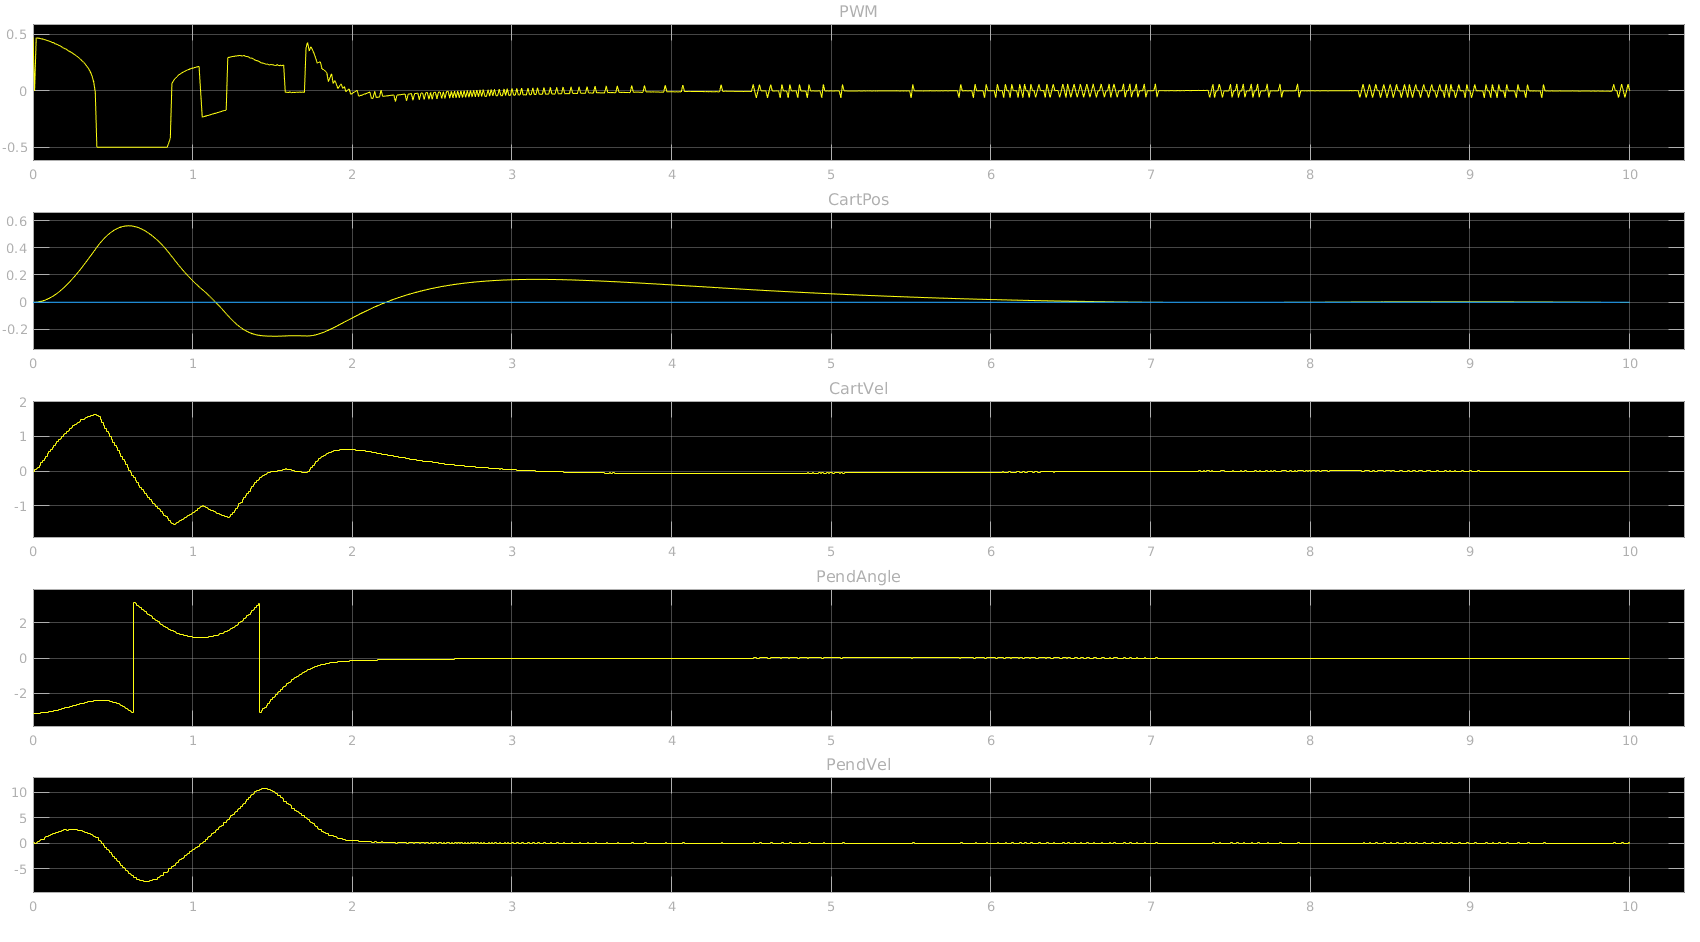
\includegraphics[width=\textwidth]{default.png}
\captionsetup{labelformat=empty}
\caption{Abb. 7-3.1: Scope des Pendels am Wagen mit Standard-LQ-Regler.}
\end{figure}




Der Regler mit $R=1$ und $Q=\text{diag}(1000, 0.1, 0.1, 0.1)$ war erfolgreich.
\begin{figure}[H]
\centering
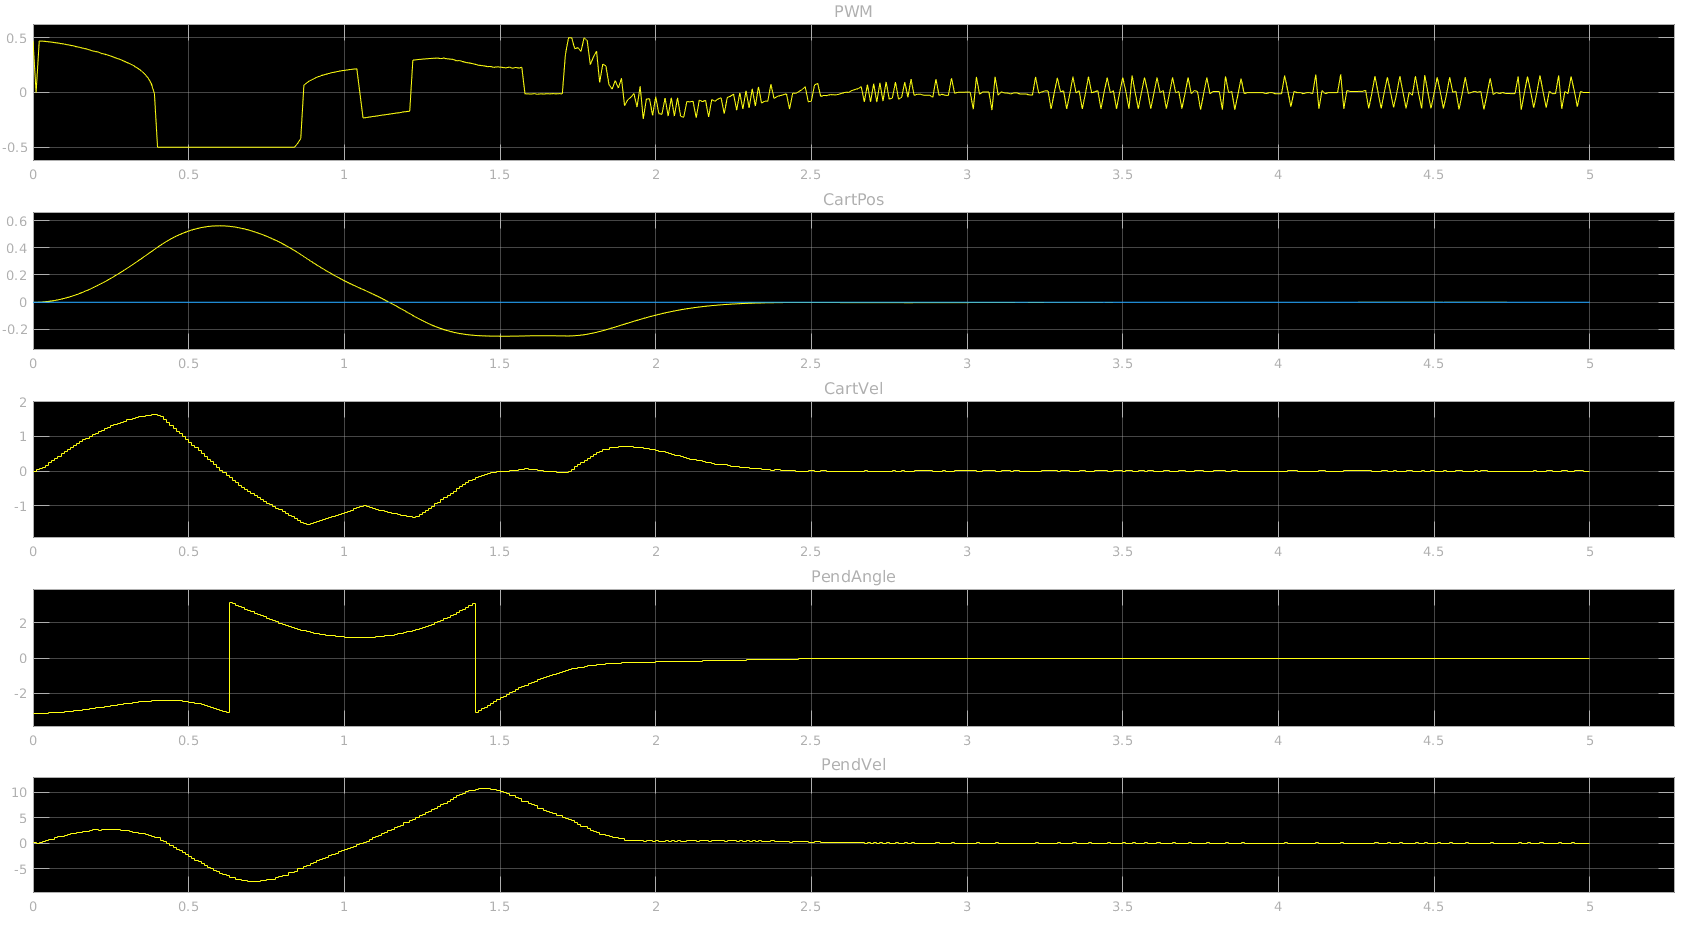
\includegraphics[width=\textwidth]{optimal.png}
\captionsetup{labelformat=empty}
\caption{Abb. 7-3.2: Scope des Pendels am Wagen mit schnellem LQ-Regler.}
\end{figure}

\end{document}
